\documentclass[12pt]{article}
\usepackage[utf8]{inputenc}
\usepackage{graphicx}
\usepackage[a4paper,width=150mm,top=25mm,bottom=25mm]{geometry}

\title{Statement of Quality Requirements}
\author{Ctrl Alt Defeat}

\begin{document}
\begin{titlepage}
    \centering



    \vspace{2cm}
    \hrulefill\\
    \vspace{1cm}
    {\Huge\bfseries SRS Documentation v3.0}

    \vspace{1cm}

    {\Large Software Requirements Specification Document for\\Domain Pulse}\\
    \vspace{1cm}
    \hrulefill\\

    \vfill

    {\large Ctrl Alt Defeat}

    \vspace{1cm}

    {\large 2023/07/31}\\
    %    \vspace{1cm}
    %    \vspace{1cm}
    %    
\includegraphics[width=10cm]{../../Images/dpLogo.png}
    %    \vspace{1cm}\\
    %    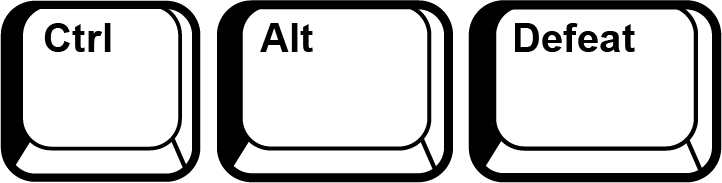
\includegraphics[width=6cm]{../../Images/cadLogo.png}

\end{titlepage}


\tableofcontents
\newpage

\newpage
\section{Quality Requirements}
While almost every possible quality requirement is something that should be aimed for as a general rule, we have identified five quality requirements most important for our system. The quality requirements below are listed in order from the most to "least" prioritised.

\subsection{Usability}
The most essential quality requirement of our system is usability. The target user for our application is not necessarily someone with high proficiency with software systems, sentiment analysis and natural language processing, or IT in general (ex: social media managers, small business and restaurant owners, etc) - consequently, the systems needs to be intuitive and non-overwhelming, both in the user interface as well as in the numerical metrics provided. As such, the following measurable requirements must be met (and can be tested by asking a non-IT person to try use the system)
\begin{itemize}
    \item Independently (ie: without any developer instruction but with the aid of a user manual / help page) and within a time of 10 minutes, a user should be able to do the following: \begin{itemize}
        \item Add a domain
        \item Add two or more sources to that domain (of any static type - ie: excluding live review)
        \item Change their site theme and profile picture
        \item Read and interpret (to a relevant extent) the data dashboard
    \end{itemize}
    \item After a further 15 minutes, a user should be able to do the following \begin{itemize}
        \item View and understand (at a high level) every visualization for every metric
        \item Create a live review and make a test review from their smartphone
        \item Generate a report of the sentiment
    \end{itemize}
    \item Additionally, the following "maximum number of clicks" requirements must be enforced \begin{itemize}
        \item Creating a new domain - 3 clicks
        \item Adding any source to any domain - 3 clicks
        \item Navigating to an arbitrary metric of a arbitrary source from any location on the app - 4 clicks
        \item Generating a report for any domain (given the user has already selected the domain) - 1 click
        \item Navigating to a specific visualization for an arbitrary source or domain from any arbitrary dashboard - 6 clicks
        \item Navigating to the help page from any arbitrary dashboad - 2 clicks
    \end{itemize}
\end{itemize}

\subsection{Security}
As will be explained below, our system will be hosted on a virtual machine on a public IP address - experience and measuring has shown that the network of computers on which the virtual machine lies is subject to up to 17 000 cyber-attacks every 24 hours. Consequently, the security of the system needs to be state of the art in order to prevent would-be attackers from wreaking havoc upon the system. To measure the strength of our security, the following requirements must be met:
\begin{itemize}
    \item No user that interacts with the system may access the profile or domain/source data of another user
    \item Should the database be leaked, all password data must be hashed to obfuscate sensitive password information
    \item The system should be immune (to the most reasonable, state-of-the-art extent possible) to the following attacks: CSRF, SQL injection, and clickjacking
    \item No user shall have the ability to make any modification to the system (ie: there will be no admin or super user)
\end{itemize}
\subsection{Performance}
Performance is an important quality requirement of our system. Our system includes a high degree of data processing and analysing (which can be a time-intensive activity) in addition to the ability to fetch data from external sources (which can also add precious seconds to execution time). Slow performance ruins the user's experience (pertaining to usability) and renders the app more frustrating that useful. Consequently, the following measurable requirements must be realised:
\begin{itemize}
    \item When a user refreshes a source, the total time taken for the data to be retrieved from an external API, preprocessed, analysed, aggregated, and returned to the user must never exceed 30 seconds, regardless of the source type and number of review fetched.
    \item When a user performs any other action that requires any other database interaction (namely: profile changes, accessing exisiting sentiment data, performing CRUD operations on domains and sources), the total time taken for the data to queried and returned to the user cannot exceed 5 seconds.
    \item The total time taken for a report to be generated cannot exceed 8 seconds, regardless of the number of sources in the domain
    \item When submitting a live review, the review need to be either successfully submitted or produce a failure message within 6 seconds.
    \item When creating a live review source, from confirming the addition of the new source, it must not take longer than 3 seconds for the QR code to become available.
\end{itemize}
\subsection{Scalability}
Scalability goes somewhat hand in hand with performance in that the system should not become overly encumbered (resulting in slower performance) when a high number of users are interacting with the system. To measure whether this is attained, the following requirements must be observed:
\begin{itemize}
    \item When the system has 50 concurrent users, the performance metrics specified above cannot exceed 1.1 times their normal threshold time
    \item When the system has 100 concurrent users, the performance metrics specified above cannot exceed 1.2 times their normal threshold time
    \item When the system has 500 concurrent users, the performance metrics specified above cannot exceed 1.5 times their normal threshold time
\end{itemize}
\subsection{Modifiability}
Ideally, this system will be useful to a fair number of people, who will in turn provide feedback for functionality, sources, and metrics they would like to be able to investigate using the system. Consequently, modifiability of the system is a desirable quality requirement in order to ensure the continuous growth and evolution of the system. Modifiability in this cases is to be defined by the following measurables:
\begin{itemize}
    \item It should not require more than 24 total work hours to add a new type of source for analysis (ex: Twitter or Reddit)
    \item It should not require more than 15 total work hours to add a new metric/statistic to be included in the analysis
    \item It should not require more than 10 total work hours to add a new type of visualization for a particular statistic
    \item Changing database for any service should not exceed more than 10* total work hours (*though this is dependent on the type and amount of data to be transferred)
\end{itemize}


\end{document}